\begin{figure*}[thb!]
  \centering
  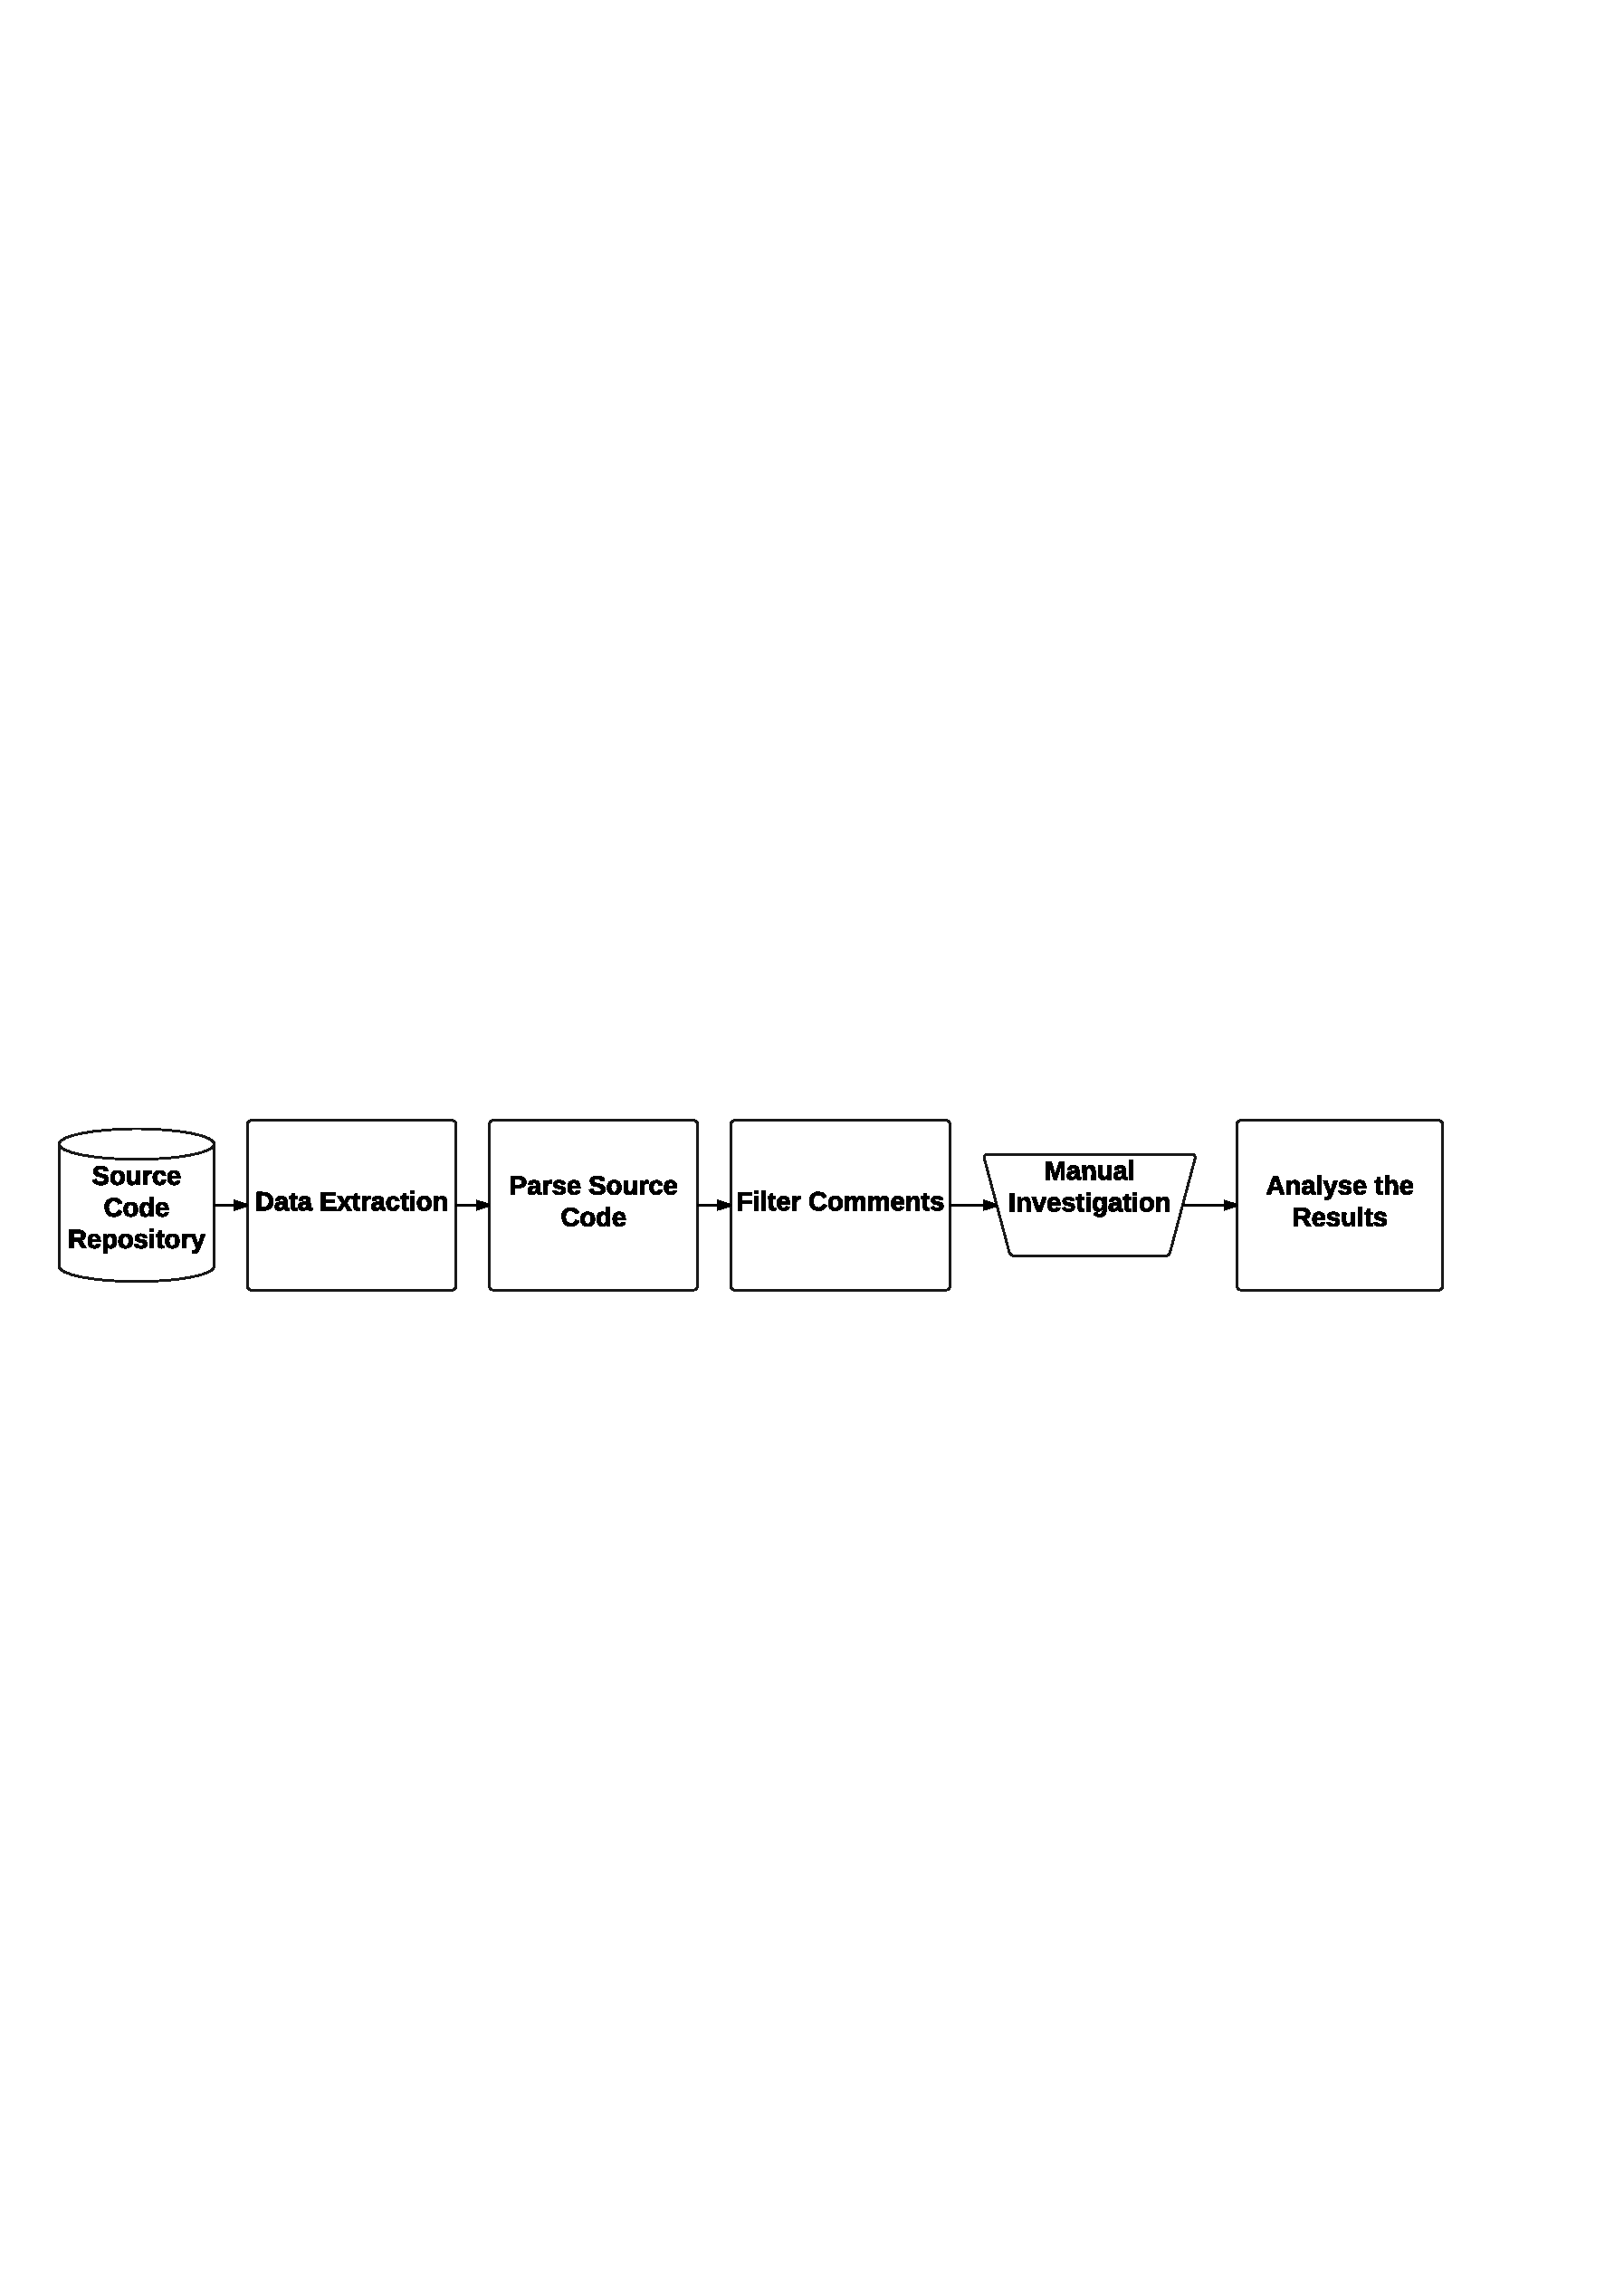
\includegraphics[width=1\textwidth]{figures/Approach}
  \caption{Approach overview}
  \label{fig:approach}
\end{figure*}

\begin{table*}[!hbt]
      \begin{center}
            \caption{Project Details}
            \label{tab:project_details}
            \begin{tabular}{l| c c r c c }
            \toprule
            \textbf{Project}   & \textbf{Release}  & \textbf{\# of classes}   & \textbf{SLOC}    & \textbf{\# of comments}  & \textbf{\# of contributors} \\ \midrule 
              Apache Ant       & 1.7.0             &  1,475                   & 115,881          & 21,587                   & 74  \\                       
              Apache Jmeter    & 2.10              &  1,181                   &  81,307          & 20,084                   & 33  \\                         
              ArgoUML          & 0.34              &  2,609                   & 176,839          & 67,716                   & 87  \\               
              Columba          & 1.4               &  1,711                   & 100,200          & 33,895                   & 9   \\                   
              JFreeChart       & 1.0.19            &  1,065                   & 132,296          & 23,474                   & 19  \\ \bottomrule
            \end{tabular}
      \end{center}
\end{table*}

The main goal of our study is to identify and quantify the different types of self-admitted technical debt found in source code comments. Figure \ref{fig:approach} shows an overview of our approach, and the following subsections detail each step of it.

\subsection{Project Data Extraction} % (fold)
\label{sub:project_data_extraction}
\revtwo{This section describes the projects that were chosen to perform the study, rather than the data extraction process [medium]}
To perform our study, we obtain the source code of five open source projects, namely Apache Ant, Apache Jmeter, ArgoUML, Columba and JFreeChart. We chose the aforementioned projects, since they belong to different application domains, and vary in size (e.g., SLOC), and in the number of contributors.

Table \ref{tab:project_details} provides statistics about each one of the projects used in our study. We provide details about the release used, the number of classes, the total source lines of code (SLOC), the total extracted comments and the number of contributors. A source line of code contain at least one valid character, which is not blank spaces or source code comments. In our study, we only use the Java files to calculate the SLOC, and to do so, we use the tool SLOCCount \cite{wheeler2004:home}. 

The number of contributors was extracted from OpenHub, an on-line community and public directory that offers analytics, search services and tools for open source software \cite{Openhub:home}. It is important to notice that the number of comments shown for each project does not represent the number of commented lines, but rather the number of individual line, block, and Javadoc comments. In total, we obtained more than 166,756 comments, found in 8,041 Java classes.
% subsection data_extraction (end)
 
\subsection{Parse Source Code} % (fold)
\label{sub:parse_source_code}
\revtwo{This section should be more detailed (including information about JDeodorant), try to make it self-contained [medium]}
After obtaining the source code of all projects, we extract the comments from their source code. We use JDeodorant \cite{Tsantalis2008CSMR}, an open-source Eclipse plug-in, to parse the source code and extract the code comments. Once extracted, we store all comments in a relational database to facilitate the processing of the data. 
% subsection parse_source_code (end) 

\subsection{Filter Comments} % (fold)
\label{sub:filter_comments}

Source code comments can be used for different purposes in a project like giving context, as part of the documentation, to express thoughts, opinions and authorship, and in some cases, to remove source code from the program. Comments are used freely for developers and with few formalities, if any at all. This informal environment allows developers to bring to light opinions, insights and even confessions (e.g., self-admitted technical debt). 

As shown in prior work by Potdar and Shihab \cite{Potdar2014ICSME}, part of these comments can be identified as self-admitted technical debt, but they are not the majority of cases. With that in mind, we develop and apply 4 filtering heuristics to narrow down the comments eliminating the ones that are less likely to be classified as self-admitted technical debt.

To do so, we developed a Java based tool that reads from the database the data obtained by parsing the source code. Next, it executes the filtering heuristics and stores the result back in the database. The retrieved data contains information like the line number that a class/comment begins/ends and the type, considering the Java syntax, of the comment (i.e., Block, Single-line or Javadoc). With this information we process the filtering heuristics as described next.

\revone{Remove only license commens instead of all of class comments [medium]}
We found that license comments are very not likely to contain self-admitted technical debt, and that license comments are commonly added before the declaration of the class. Therefore, we create a heuristic that removes comments that are placed before the class declaration. Since we know the line number that the class was declared we can easily check for comments that are placed before that line and remove them.

We also notice that some times developers make long comments, using multiple \emph{single-line} comments instead of a Block comment. This characteristic can hinder the understanding of the message. Consider the case that the reader (i.e., human or machine) analyze each one of these comments independently, the message would be incomplete and the meaning lost. To solve that problem, we create a heuristic that searches for consecutive single-line comments and groups them as one. We identify consecutive comments by subtracting the line number of both comments. If the result of the difference is equals a -1 we have a consecutive comment. For example, Single-line comment A is placed in line number 100 and Single-line comment B is placed in line 101. The subtraction of the line numbers will result in -1, therefore the comments are consecutive.
 
\revone{Add regular expression used for removing java source code [easy]}
Similarly, is common to find commented source code across the projects, and this can be due to many different reasons. One of the possibilities is that the code is not being used, other is that the code is used for debug purposes only. Based on our analysis, commented source code does not have self-admitted technical debt. Our heuristic remove commented source code using a simple regular expression that captures typical Java code structures.

% else\s*\{|try\s\{|do\s*\{|finally\s*\{|if\s*\(|for\s*\(|while\s*\(|switch\s*\(|Long\s*\(|Byte\s*\(|Double\s*\(|Float\s*\(|Integer\s*\(|Short\s*\(|BigDecimal\s*\(|BigInteger\s*\(|Character\s*\(|Boolean\s*\(|String\s*\(|assert\s*\(|System.out.|public\s*void|private\s*static*final|catch\s*\( 


Lastly, when analyzing Javadoc comments we found that they rarely mention self-admitted technical debt. For the Javadoc comments that does mention self-admitted technical debt we notice that they usually contains one of the task-reserved words (i.e., ``todo'', ``fixme'', or ``xxx''). Based on this, our heuristic remove all comments of the type Javadoc unless they contain at least one of the task-reserved words. To do so, we create a simple regular expression that search for the task-reserved words before removing the comment.  

The steps mentioned above significantly reduced the number of comments in our dataset and helped us focus on the most applicable and insightful comments. For example, in the Apache Ant project, applying the above steps helped reduce the number of comments from 21,587 to 4,140 comments meaning that 19.17\% of the comments were kept for analysis. Table \ref{tab:filtering_heuristics_details} provides details for each one of the projects.

\begin{table}[!hbt]
      \begin{center}
            \caption{Filtering heuristics details}
            \label{tab:filtering_heuristics_details}
            \begin{tabular}{l| p{0.55in} p{0.75in} p{0.75in} }
            \toprule
            \thead{\textbf{Project}}   & \textbf{Total \# of comments}  & \textbf{\# of comments after filtering} & \textbf{\%  of TD-related comments}\\ \midrule 
              Apache Ant       & 21,587                & 4,140                   & 19.17 \% \\ 
              Apache Jmeter    & 20,084                & 8,163                   & 40.64 \% \\
              ArgoUML          & 67,716                & 9,788                   & 14.45 \% \\              
              Columba          & 33,895                & 6,569                   & 19.38 \% \\
              JFreeChart       & 23,474                & 4,436                   & 18.89 \% \\ \bottomrule
            \end{tabular}
      \end{center}
\end{table}
% subsection filter_comments (end)

\subsection{Manual Classification} % (fold)
\label{sub:manual_classification}
\revtwo{Clarify how the developed tool provides a list of possible classifications [easy]}
To manually classify the comments we first developed a Java based tool that show one comment at time and gives a list of possible classifications  that will be assigned to the comment~\cite{Alves2014MTD}. After applying the different filtering steps, we successfully classified 33,093 comments. The more than 33 thousand comments were classified into five different types of self-admitted technical debt, i.e., design debt, defect debt, documentation debt, requirement debt and test debt.

The first author who made the classification has more than 8 years of experience working in the industry as a software engineer, during this time he designed, implemented and maintained several programs using, in particular the Java programming language. He developed solid skills in object orientated programming and design patterns. We consider that these qualifications provide the necessary background to conduct the manual classification of the comments.   
% subsection manual_classification (end)
